\subsection{Customizar o Asterisk}

A customização do Asterisk será fundamental para realizar a comunicação entre os sistemas, sendo responsável em disponibilizar de forma padronizada o acesso a URA no atendimento de primeiro nível de todas as chamadas recebidas, e disparar solicitações a recursos externos conforme a necessidade do cliente que efetuou a ligação.
Primeiramente iremos configurar um ramal, utilizando a interface web do Disc-os, conforme exemplo abaixo na figura \ref{figura:cadastroRamapSIP}:


\begin{figure}[!htb]
	\centering
	\caption{Cadastro de um Ramal SIP.}	
	\label{figura:cadastroRamapSIP}
	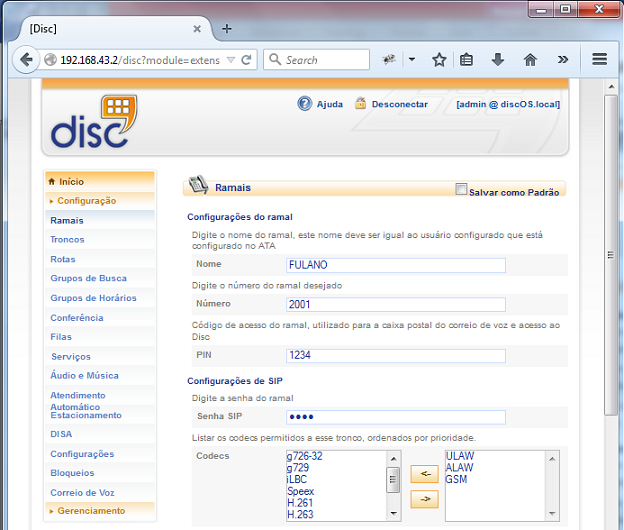
\includegraphics{figuras/cadastro_ramal_sip.png}
	\legend {\fontsize{10}{12}\selectfont {Fonte: Autoria Própria}.}
\end{figure}


Conforme visto acima, está sendo configurado o ramal de número 2001, com o nome de FULANO e definido alguns \textit{codecs} que serão permitidos utilizar neste ramal, após isto o Disc-OS se encarregará de alterar o arquivo de propriedades \textit{sip.conf} inserindo o ramal desejado com as características informadas.
Para a configuração da Unidade de Resposta Audível, será preciso definir claramente quais serão as opções disponíveis e quais serão as possíveis saídas com o seus devidos tratamentos, neste trabalho foi desenvolvido um fluxo de atendimento próprio, demonstrado na figura \ref{figura:fluxoURA}: 

\begin{figure}[!htb]
	\centering
	\caption{Diagrama do Fluxo da Unidade de Resposta Audível}
	\label{figura:fluxoURA}	
	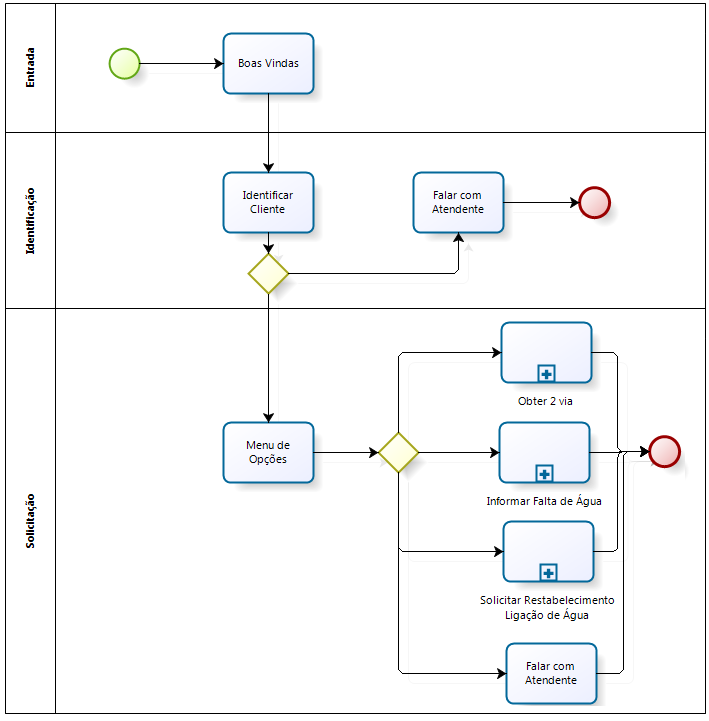
\includegraphics{figuras/fluxo_ura.png}
	\legend {\fontsize{10}{12}\selectfont {Fonte: Autoria Própria}.}
\end{figure}


Dessa forma o cliente terá a opção de falar com o atendente logo no primeiro menu de atendimento e nos demais sub-fluxos, comportamento exigido conforme o artigo 4 da Lei nº 8.078 \cite{leiAtendimentoAoConsumidor}, que fixa normas gerais sobre o Serviço de Atendimento ao Consumidor, após realizar o passo de identificação o mesmo terá acesso as opções de serviços automatizados via integração caso ocorra tudo com êxito, caso não seja possível identificar o cliente será redirecionado para o Falar com Atendente.
A interface \textit{Web} do Disc-OS permite realizar a configuração da URA, de forma bem intuitiva, inclusive definir tempos de espera, direcionamento para outros Ramais entre outras configurações que tornam o processo de configuração muito mais prático, no entanto para configurar o fluxo da URA realizando a comunicação via AGI com o \textit{Middleware} será preciso realizar o procedimento manual de configuração, segue abaixo a configuração utilizada para criação do contexto de PESQUISAR\_CLIENTE utilizada para identificar o cliente, descrito no arquivo \textit{/etc/asterisk/extensions.conf}, conforme representado pelo algoritmo 2 abaixo:


\textbf{Algoritmo 2} – Fluxo de identificação do cliente (Asterisk). \\
\textbf{Entrada}: Recebe a chamada atual com prioridade um.
\begin{enumerate}
	\item $atenderLigação() \hspace{20 mm} \triangleright recepciona a ligação$
	\item $tocarAudio(beep)  \hspace{20 mm} \triangleright	tocar áudio de aviso$
	\item $tempo\_limite\_discagem \longleftarrow 3 \hspace{20 mm} \triangleright defini tempo limite de espera entre dígitos $		 
	\item $tempo\_limite\_resposta \longleftarrow 7 \hspace{20 mm} \triangleright defini tempo limite de espera do primeiro digito$
	\item $digitos  \longleftarrow lerDigitos() \hspace{20 mm} \triangleright ler os dígitos informados $
	\item $canal [cliente]  \longleftarrow dígitos  \hspace{20 mm} \triangleright adiciona os dígitos no canal  $
	\item $Agi(pesquisar.imovel.cliente.agi)  \hspace{20 mm} \triangleright faz a chamada agi $
	\item \textbf{se} $canal [situacao] == sucesso  \hspace{10 mm} $ \textbf{então}
	\item \hspace{7 mm}$gotoSucesso() \hspace{20 mm} \triangleright redireciona a ligação para sucesso $
	\item \textbf{senão}
	\item \hspace{7 mm}$ gotoContextoAtendente() \hspace{20 mm} \triangleright redireciona a ligação para falar com atendente $					
	\item \textbf{fim}
\end{enumerate}


Neste trecho é declarado o contexto [PESQUISAR\_CLIENTE], cuja prioridade 1 será anteder a ligação e logo em seguida emitir um áudio chamado beep, foi defini o tempo limite de espera para o primeiro dígito de 7 segundos e o tempo limite de espera para a discagem dos dígitos de 3 segundos, será lido os valores informados pelo Originador da chamada e atribuída a variável CLIENTE\_IMOVEL, após isto será realizada uma requisição via interface de comunicação  AGI para o \textit{Middleware}, solicitando o serviço mapeando em pesquisar.imovel.cliente.agi, dependendo do retorno deste serviço será realizado um redirecionamento da ligação para um contexto específico, para consultar a configuração completa da URA encontra-se disponível nos anexos deste trabalho.
Para tanto, será necessário customizar os arquivos de áudio para serem tocados, conforme as operações disponíveis forem acessadas. Para efetuar a gravação do áudio foi utilizado um recurso do Asterisk, discando para *77, existe um contexto que utiliza aplicativos nativos para realiza a gravação no formato WAV e o disponibiliza no diretório \textit{/var/lib/asterisk/sounds/custom/} para utilização.
Após as configurações básicas, será preciso ter um dispositivo para efetuar as chamadas e conseguir se comunicar com a URA, neste cenário existe um recurso chamado de \textit{Softphone}, são programas que tornam o computador em um Ramal IP, possibilitando realizar e receber chamadas, com essa finalidade foi utilizado o Zoiper\footnote{Disponível em \url{https://www.zoiper.com/}}, conforme visto na figura \ref{figura:zoiper}:

\begin{figure}[!htb]
	\centering
	\caption{Softphone Zoiper sendo executado}	
	\label{figura:zoiper}
	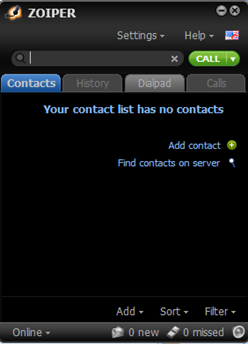
\includegraphics{figuras/zoiper.png}
	\legend {\fontsize{10}{12}\selectfont {Fonte: Autoria Própria}.}
\end{figure}


Para adicionar o ramal é preciso definir qual será o protocolo utilizado e inserir os dados configurados no Asterisk conforme visto na figura \ref{figura:zoiperConfigRamal} abaixo:

\begin{figure}[!htb]
	\centering
	\caption{Configurar Ramal no Zoiper}
	\label{figura:zoiperConfigRamal}
	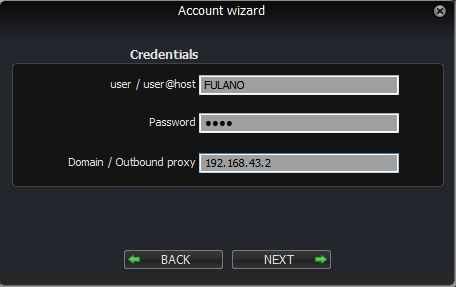
\includegraphics{figuras/configurar_ramal_zoiper.png}
	\legend {\fontsize{10}{12}\selectfont {Fonte: Autoria Própria}.}
\end{figure}

Após realizar todos estes passos será possível acessar os serviços disponibilizados pela URA, através do Zoiper efetuar as chamadas para percorrer os fluxos previamente definidos.